\section{Desarrollo}\label{sec:desarrollo}

Se realizó el siguiente diagrama para entender la lógica del programa.
%%%%%%%%%DIAGRAMA DE FLUJO

\begin{figure}[H]
    \centering
    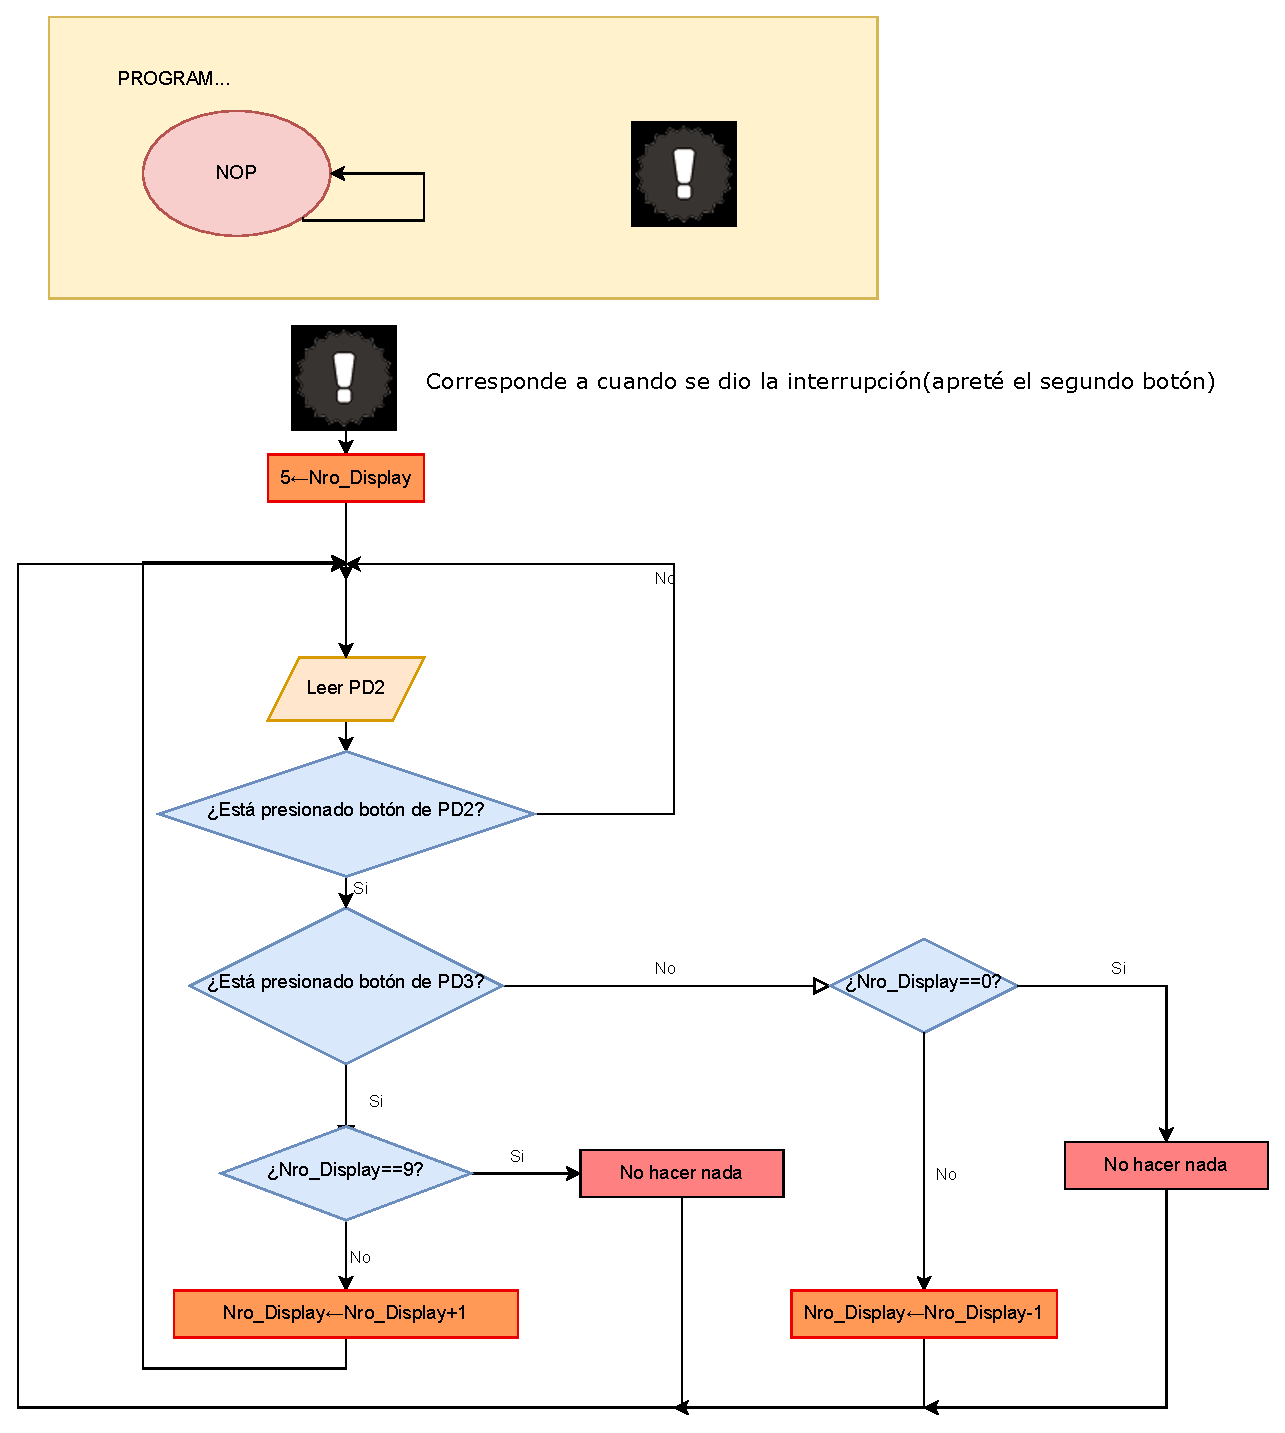
\includegraphics[width=\linewidth]{imagenes/tp2.eps}
    \caption{Diagrama de Flujo}
    \label{fig:CIRCRECT1}
\end{figure}
%%%%%%%%%

Los materiales usados fueron: 

\begin{itemize}
    \item 1 display de 7 segmentos
    \item 2 Pulsadores
    \item 7 Resistencias de 220 Ohms
    \item Cables puente macho-macho
    \item Arduino UNO
    \item Cable para conectar Arduino con PC
\end{itemize}

Los valores para las resistencias fueron elegidos en base a que la corriente máxima en directa que circula por los led del 7 segmentos no debe superar los 20 mA y la tensión en directa en estos es de 1,8V según la hoja de datos. Si a los led se los alimenta con 5V entonces la resistencia que debemos elegir debe ser de 160 Ohm (sale de circular la malla) y elegí la resistencia de 220 Ohm porque era la de valor comercial más próxima a ese valor que tenía a disposición.

El Trabajo práctico preguntaba que pasa si en vez de colocar siete resistores se coloca uno solo en el nodo común. La respuesta a esto es que nos queda el siguiente circuito:
%%%%%%%%%circuito con diodos

\begin{figure}[H]
    \centering
    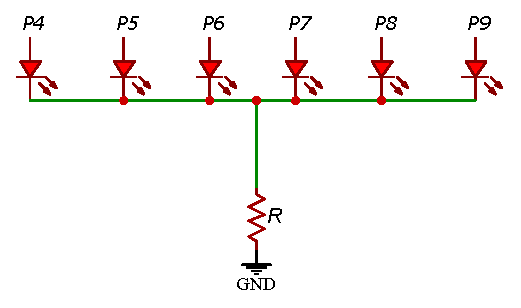
\includegraphics[width=.5\linewidth]{imagenes/DIODOS.eps}
    \caption{Circuito de los diodos con una R común}
    \label{fig:diodos}
\end{figure}
%%%%%%%%%



En el caso que los 7 diodos estén prendidos tendremos una $I_D=20\,mA$ como máximo y un $V_D=1,8\,V$ entonces la resistencia debería de ser al hacer la cuenta de 23 Ohm.

Ahora, el caso que tenga un diodo solo prendido, la corriente que circule por ese diodo será: 
$I_D(caso 1)=(5V-1,8V)/R$ y con esa R calculada se me quemaría el diodo ya que sería mayor a 20 mA. Lo que me conviene es asegurarme de que en el caso límite(que es este, donde cae más corriente en un diodo), no se me queme, para eso pido que R sea mínimo la R calculada para el caso que están las 7 resistencias, es decir, 220 Ohm(porque es el valor comercial que conseguí).
Ahora bien, con ese valor de resistencia, si tengo prendido un Led, circulan 20 mA, ¿Qué pasa si prendo más de un Led? Esa corriente se distribuye por los diodos encendidos (por ley de nodos), si tengo 2 leds prendidos la corriente en cada diodo va a ser de 10 mA, si tengo 4 prendidos de 5mA y así hasta llegar a los 7 prendidos. 
¿Qué pasa entonces? Que al circular menos corriente, la intensidad de la luz en los diodos en consecuencia va a ser menor y no me va a servir para nada.

Se me ocurre una forma de aprovechar recursos: Podría prender un led por vez durante un período de tiempo muy corto de manera que al ojo humano, se vea que están prendidos todos los led (aunque en realidad no lo estén). De esta forma podría usar una resistencia sola pero debería ir prendiendo y apagando los puertos uno por uno cada (por ejemplo) 10ms de manera que siempre se vean todos prendidos a la vista.

Contestando la pregunta dos, para cada pin se puede entregar $I_{OH}=-I_{OL}=20\,mA$ en estado estable con una fuente de 5V (según la hoja de datos del micro).
Cada pin de E/S puede soportar picos de corriente de hasta 40 mA.
La corriente por cada puerto no debe superar los 200 mA en el ATMega328.

Para ser más específicos:
\begin{itemize}
    \item La suma de toda la corriente en HIGH (source) para los puertos C0 – C5, D0 – D4, ADC7, RESET no debe exceder los 150 mA
    \item La suma de toda la corriente en HIGH (source) para los puertos B0 – B5, D5 – D7, ADC6, XTAL1, XTAL2 no debe exceder los 150 mA.
    \item Si la corriente en HIGH supera los valores nominales, el voltaje en HIGH puede superar los valores nominales. No se garantiza que los pines puedan dar más corriente que la de los valores de test.
    \item La suma de toda la corriente en LOW (sink) para los puertos C0 – C5, ADC7, ADC6 no debe exceder los 100 mA
    \item La suma de toda la corriente en LOW (sink) para los puertos C0 – C5, ADC7, ADC6 no debe exceder los 100 mA
    \item La suma de toda la corriente en LOW (sink) para los puertos B0 – B5, D5 – D7, XTAL1, XTAL2 no debe exceder los 100 mA
    \item La suma de toda la corriente en LOW (sink) para los puertos  D0 – D4, RESET no debe exceder los 100 mA
    \item Si la corriente en LOW supera los valores de test, el voltaje de LOW puede exceder los valores nominales. No se garantiza que los pines puedan obtener (sink) más corriente que la de los valores de test.
\end{itemize}


\begin{figure}[H]
    \centering
    \includegraphics[width=.6\linewidth]{imagenes/Atmega 328 absolute maximum ratings.PNG}
    \caption{Valores datasheet para tensiones y corriente máximas}
    \label{fig:diodos}
\end{figure}
%%%%%%%%%

 Si en el programa se eliminase el manejo por la interrupción del pin PD2 y se quisiera
conseguir, no obstante, que el programa siga funcionando de la misma forma, lo que haría sería consultar constantemente si se cambió el estado del PIN2, lo cual lo vuelve ineficiente.

\section{Código del programa}
El código del programa es el siguiente. Muchas cosas aparecen negadas dado que el 7 segmentos que terminé utilizando era ánodo común.
Para evitar los rebotes decidí realizar un delay de 200ms. El tiempo lo elegí considerando el rebote que se generaba. Otra solución para este problema hubiera sido colocar un capacitor, ambas soluciones son eficientes pero con el delay implementado nos ahorramos un componente del circuito, con el costo de realizar más operaciones.

\begin{verbatim}
    /*
 * tp27seg.asm
 *
 *  Created: 23/05/2021 09:40:54 p.m.
 *   Author: Vero
 */ 
 
.MACRO READ_TABLE // (Rxx, table, offset)
  push ZL
  push ZH
  push R29
  ldi  ZL, low(@1*2)    // low byte of table adr to r30
  ldi  ZH, high(@1*2)   // high byte of table adr to r31
  //adiw ZL, @2           // add offset 
  add ZL, @2
  ldi R29, 0
  adc ZH, r29
  lpm @0, Z            // read byte
  pop R29
  pop ZH
  pop ZL
.ENDMACRO 

.equ SEG7_0=0x7E
.equ SEG7_1=0x30
.equ SEG7_2=0x6D
.equ SEG7_3=0x79
.equ SEG7_4=0x33
.equ SEG7_5=0x5B
.equ SEG7_6=0x5F
.equ SEG7_7=0x71
.equ SEG7_8=0x7F
.equ SEG7_9=0X73
.equ SHIFT_L=4
.equ SHIFT_H=5
.equ MASK_L=0xF0
.equ MASK_H=0x07

.equ PORT_H=PORTB
.equ PORT_L=PORTD

.def BITS_NRO=R16
.def AUX2=R17
.def AUX3=R18
.def CONTADOR=R19

.device ATmega328P
; Vector de reset
.org 0
		rjmp Reset 
; Vector de INT0 (pin PD2) 
.org INT0addr
		rjmp EXT_INT0

Reset:	;stack
		ldi R31,low(RAMEND) 
	  	out SPL,R31
        ldi R31, high(RAMEND)
        out SPH, R31
 		
		//configurar puertos
		LDI AUX2, (MASK_H | (1<<5))
		OUT DDRB, AUX2 ;seteo el puerto B como salida y el led interno
		LDI AUX2, 0b11110000 ;MASK_L
		OUT DDRD, AUX2 ;seteo los leds del puerto D como salida
		LDI AUX2, 0xFF
		OUT PORTD, AUX2
		LDI AUX2, 0b00000111
		OUT PORTB, AUX2
		;seteo resistencias pull up
		;SBI PORTD,2
		;CBI DDRD, 3
		;SBI PORTD,3
		
		; prueba de lectura del boton en PD3
		SBI PORTB, 5 

		;inicializo interrupciones
		call INIT_IRQ_INT0

		// Inicializo 7 segmentos
		ldi CONTADOR, 5    ;Valor inicial del 7 segmentos
		READ_TABLE BITS_NRO, TABLA_7SEG, CONTADOR
		CALL WRITE_7SEG
		sei	          ; Hab. global de interrupciones

		// Bucle principal
		HANG: RJMP HANG
	/*********************************/

WRITE_7SEG: ;BITS_NRO -> PORTB, PORTD
	push AUX2
	push AUX3
	push R0
	push R1
	;Desdoblo BITS_NRO en dos partes, para escribir c/u en un puerto distinto
	MOV AUX2,BITS_NRO ;copio
	COM AUX2 ;Display catodo común?
	ANDI AUX2, 0x7F ;uso los bits 0 a 7 solamente
	;;AND AUX2,MASK_L ;aplico mascara para obtener parte baja (respectivo a PORT_L)
	LDI AUX3, 1<<SHIFT_L 
	MUL AUX2, AUX3  ;shift de SHIFT_L bits a la izq. AUX2=0bABCD_EFGH -> R1=0b0000_ABCD, R0=0bEFGH_0000 
	OUT PORTB,R1  ;escribo la parte alta en PORTH

	IN AUX3,PORTD ;leo PORTD
	LDI AUX2,~(MASK_L) 
	AND AUX3, AUX2 ; borro a 0 los bits que voy a usar de portd, dejo intacto el resto

	MOV AUX2, R0 ;copio bits a escribir en el puerto
	OR AUX3, AUX2 ;escribo unos donde habia ceros
	OUT PORTD,AUX3 ;escribo la parte baja en PORT_L

	pop R1
	pop R0
	pop AUX3
	pop AUX2
	RET

TITILAR_LED_INT:
	CBI PORTB, 5 ;titilo led interno
	CALL DELAY_ms
	SBI PORTB, 5
	CALL DELAY_ms ;espero para no contar rebotes
	CBI PORTB, 5
	RET
	
EXT_INT0: ;manejo de interrupción externa
	CALL TITILAR_LED_INT
	SBIC PIND,1 ;SALTEA LA SIGUIENTE LINEA SI HAY UN 0 EN EL PD1 === BOTON APRETADO
	RJMP DECREMENTAR

	INCREMENTAR:		
	CPI CONTADOR, 9
	BREQ FIN_EXT_INT0; si llego a 9, salgo
	INC CONTADOR ;incremento contador y busco en el array
	RJMP FIN_EXT_INT0
	
	DECREMENTAR:
	CPI CONTADOR, 0
	BREQ FIN_EXT_INT0; si llego a 0, salgo	
	DEC CONTADOR ;decremento contador y busco en el array
	
	
	;fin
	FIN_EXT_INT0:
	READ_TABLE BITS_NRO, TABLA_7SEG, CONTADOR
	CALL WRITE_7SEG
	CALL DELAY_200ms
	RETI

	
DELAY_1s: ;delay 1s
	push R18
	push R19
	push R20

	LDI R18, 82
	LDI R19, 255
	LDI R20, 255
	DELAY_1s_LOOP:
	dec R20
	brne DELAY_1s_LOOP
	dec R19
	brne DELAY_1s_LOOP
	dec R18
	brne DELAY_1s_LOOP

	pop R20
	pop R19
	pop R18
	RET

DELAY_200ms: 
	push R18
	push R19
	push R20

	LDI R18, 16
	LDI R19, 255
	LDI R20, 255
	DELAY_200ms_LOOP:
	dec R20
	brne DELAY_200ms_LOOP
	dec R19
	brne DELAY_200ms_LOOP
	dec R18
	brne DELAY_200ms_LOOP

	pop R20
	pop R19
	pop R18
	RET
/*
DELAY_ms: ;delay pequeño
	push R18
	push R19
	ldi R18, 609 ; para 8mhz
	; 1 ciclo
	LOOP0:
	ldi R19, 200 ; 1 ciclo
	LOOP1:
	dec R19 ; 1 ciclo
	brne LOOP1 ;
	dec R18 ; 1
	brne LOOP0 ; 2

	pop R19
	pop R18
	RET*/

DELAY_ms: ;delay pequeño
	push R18
	push R19
	LDI R18, 255
	LDI R19, 255
	DELAY_ms_LOOP:	
	dec R19
	brne DELAY_ms_LOOP
	dec R18
	brne DELAY_ms_LOOP

	pop R19
	pop R18
	RET

TEST_7SEG:
	LDI AUX2,MASK_H
	OUT PORTB, AUX2 ;apago todas los leds (por 1)  
	CALL DELAY_1s
	LDI AUX2, ~MASK_H
	OUT PORTB, AUX2
	CALL DELAY_1s
	LDI AUX2,MASK_H
	OUT PORTB, AUX2 ;apago todas los leds (por 1)  

	LDI AUX2,MASK_L
	OUT PORTD, AUX2 ;apago todas los leds (por 1)  
	CALL DELAY_1s
	LDI AUX2, ~MASK_L
	OUT PORTD, AUX2
	CALL DELAY_1s
	LDI AUX2,MASK_L
	OUT PORTD, AUX2 ;apago todas los leds (por 1)  
	RJMP TEST_7SEG

; Configura INT0
INIT_IRQ_INT0:
	ldi R16, (1<<ISC01)|(1<<ISC00)  ;flanco descendente	
	sts EICRA, R16					
	ldi R16, (1<<INT0)				
	out EIMSK, R16					; Habilita máscara
	RET


TABLA_7SEG:	.DB SEG7_0, SEG7_1, SEG7_2, SEG7_3, SEG7_4, SEG7_5, SEG7_6, SEG7_7, SEG7_8, SEG7_9

\end{verbatim}


